% !TeX program = xelatex
% Bien dich:  tectonic --reruns 2 slides/colpali_deep_dive.tex
%
% Deck chuyen sau ve paper ColPali (arXiv:2407.01449, ICLR 2025).
%   Phan I  : vi sao pipeline parsing la nut that
%   Phan II : kien truc, late interaction, training, chi phi, ket qua, ablation
%   Phan III: thuc nghiem retrieval tren corpus tieng Viet cua do an (CPU-only)
%
% Nguon so lieu paper: ar5iv HTML cua arXiv:2407.01449 (ban v3),
%   Table 2 (nDCG@5), Table 6 (Recall@1), Table 7 (ablation).
% Nguon so lieu do an: scripts/eval/*.py + data/eval/gold_qa.jsonl.
\documentclass[aspectratio=169,10pt]{beamer}

% ---- Font: uu tien font Windows, tu lui ve font TeX mac dinh ----
\usepackage{fontspec}
\IfFontExistsTF{Arial}
  {\setsansfont{Arial}\setmainfont{Arial}}
  {\IfFontExistsTF{TeX Gyre Heros}
     {\setsansfont{TeX Gyre Heros}\setmainfont{TeX Gyre Heros}}
     {\setsansfont{Latin Modern Sans}\setmainfont{Latin Modern Roman}}}
\IfFontExistsTF{Consolas}
  {\setmonofont{Consolas}}
  {\IfFontExistsTF{DejaVu Sans Mono}
     {\setmonofont{DejaVu Sans Mono}}
     {\setmonofont{Latin Modern Mono}}}

\usepackage{amsmath}
\usepackage{amssymb}
\usepackage{booktabs}
\usepackage{tabularx}
\usepackage{array}
\usepackage{xcolor}
\usepackage{tikz}
\usetikzlibrary{arrows.meta,positioning,calc,fit,shapes.geometric}

% --- Professional Academic Theme Settings ---
\usetheme{Boadilla}
\usecolortheme{rose}

\definecolor{navyprimary}{RGB}{15, 44, 89}
\definecolor{slateaccent}{RGB}{51, 65, 85}
\definecolor{blueaccent}{RGB}{29, 78, 216}
\definecolor{lightgraybg}{RGB}{248, 250, 252}
\definecolor{darktext}{RGB}{30, 41, 59}
\definecolor{mathred}{RGB}{185, 28, 28}
\definecolor{mathgreen}{RGB}{22, 101, 52}

\setbeamercolor{structure}{fg=navyprimary}
\setbeamercolor{title}{fg=white, bg=navyprimary}
\setbeamercolor{frametitle}{fg=white, bg=navyprimary}
\setbeamercolor{block title}{fg=white, bg=navyprimary}
\setbeamercolor{block body}{fg=darktext, bg=lightgraybg}
\setbeamercolor{block title example}{fg=white, bg=slateaccent}
\setbeamercolor{block body example}{fg=darktext, bg=lightgraybg}

\setbeamertemplate{navigation symbols}{}
\setbeamertemplate{footline}[frame number]

\newcommand{\code}[1]{\texttt{\footnotesize #1}}
\newcommand{\hot}[1]{\textcolor{mathred}{\textbf{#1}}}
\newcommand{\good}[1]{\textcolor{mathgreen}{\textbf{#1}}}
\newcommand{\E}{\mathbf{E}}

% --- Metadata ---
\title[Kiến trúc Chuyên sâu ColPali]{\textbf{Kiến trúc Chuyên sâu ColPali:\\ Efficient Document Retrieval with Vision Language Models}}
\subtitle{Bóc tách Toán học, Biểu diễn Tensor, Cơ chế Huấn luyện \& Pipeline Triển khai}
\author[Báo cáo Chuyên sâu AI]{Báo cáo Kỹ thuật Chuyên đề: Vision-Language Models in IR}
\institute[Advanced AI Lab]{Phòng Thí nghiệm Trí tuệ Nhân tạo \& Xử lý Ngôn ngữ Tự nhiên}
\date{\today}

\begin{document}

% =============================================================
% SLIDE 1: TITLE
% =============================================================
\begin{frame}
  \titlepage
\end{frame}

% =============================================================
% SLIDE 2: AGENDA
% =============================================================
\begin{frame}{Nội dung Báo cáo Chuyên sâu}
  \begin{columns}[T]
    \begin{column}{0.48\textwidth}
      \begin{block}{Phần I: Giới hạn của Pipeline Parsing}
        \begin{itemize}
          \item Phân tích sai số tích lũy (error cascading)
          \item Mất mát thông tin cấu trúc 2 chiều
          \item Chi phí indexing của OCR/captioning
        \end{itemize}
      \end{block}
      \begin{block}{Phần II: Cấu trúc Mô hình ColPali}
        \begin{itemize}
          \item SigLIP Vision Encoder \& patch tokenization
          \item Linear projection \& Gemma-2B
          \item Late interaction (MaxSim) \& hàm mất mát
          \item Huấn luyện, chi phí, kết quả ViDoRe
        \end{itemize}
      \end{block}
    \end{column}
    \begin{column}{0.48\textwidth}
      \begin{block}{Phần III: Thực nghiệm trên corpus tiếng Việt}
        \begin{itemize}
          \item Thiết kế: 7 PDF, 27 trang, 130 câu hỏi
          \item Baseline BM25 / row-JSON / ColPali
          \item Recall@$k$, MRR ở mức trang
        \end{itemize}
      \end{block}
      \begin{block}{Phần IV: Kết luận \& Hướng tiếp}
        \begin{itemize}
          \item Khi nào nên (và không nên) dùng visual retrieval
          \item Fine-tune LoRA tiếng Việt, patch $\rightarrow$ bounding box
        \end{itemize}
      \end{block}
    \end{column}
  \end{columns}

  \vspace{2mm}
  \begin{center}
    \footnotesize
    Paper: Faysse et al., \emph{ColPali: Efficient Document Retrieval with Vision Language Models}, ICLR 2025 (arXiv:2407.01449)
  \end{center}
\end{frame}

% =============================================================
% SLIDE 3: VI SAO PARSING LA NUT THAT
% =============================================================
\begin{frame}{Vì sao pipeline parsing là nút thắt?}
  \centering
  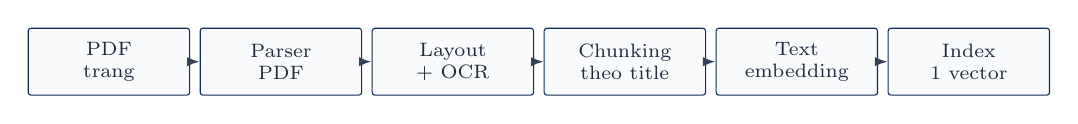
\begin{tikzpicture}[
      node distance=1.2mm,
      box/.style={draw=navyprimary, fill=lightgraybg, rounded corners=1pt,
                  minimum width=2.05cm, minimum height=0.85cm, align=center,
                  font=\scriptsize, text=darktext},
      arr/.style={-{Latex[length=1.6mm]}, draw=slateaccent, thick}]
    \node[box] (pdf) {PDF\\trang};
    \node[box, right=of pdf] (par) {Parser\\PDF};
    \node[box, right=of par] (lay) {Layout\\+ OCR};
    \node[box, right=of lay] (chk) {Chunking\\theo title};
    \node[box, right=of chk] (emb) {Text\\embedding};
    \node[box, right=of emb] (idx) {Index\\1 vector};
    \draw[arr] (pdf) -- (par);
    \draw[arr] (par) -- (lay);
    \draw[arr] (lay) -- (chk);
    \draw[arr] (chk) -- (emb);
    \draw[arr] (emb) -- (idx);
  \end{tikzpicture}

  \vspace{1mm}
  {\footnotesize\itshape Mỗi mũi tên là một nguồn lỗi; lỗi tích lũy (error cascading) theo chiều dài pipeline.}

  \vspace{3mm}
  \begin{columns}[T]
    \begin{column}{0.32\textwidth}
      \begin{block}{\small Bảng không kẻ}
        \footnotesize
        Parser dựa trên đường kẻ/whitespace: mất hàng, lệch cột, gộp 2 bảng song song.
      \end{block}
    \end{column}
    \begin{column}{0.32\textwidth}
      \begin{block}{\small Cấu trúc 2 chiều}
        \footnotesize
        Vị trí, font, màu, đường bao mang nghĩa. Chunk văn bản 1D xóa mất các tín hiệu này.
      \end{block}
    \end{column}
    \begin{column}{0.32\textwidth}
      \begin{block}{\small Chi phí}
        \footnotesize
        OCR/captioning: hàng chục giây/trang; khó scale lên triệu trang.
      \end{block}
    \end{column}
  \end{columns}

  \vspace{1mm}
  \begin{center}
    \footnotesize
    Kết luận của paper: \emph{tối ưu pipeline ingestion} mang lại nhiều điểm hơn \emph{tối ưu embedding model} (Table~2).
  \end{center}
\end{frame}

% =============================================================
% SLIDE 4: BANG CHUNG DINH LUONG
% =============================================================
\begin{frame}{Bằng chứng định lượng: cùng benchmark, khác pipeline}
  \centering
  \footnotesize
  \begin{tabular}{@{}lcccc@{}}
    \toprule
    Hệ thống (ViDoRe, TB 10 task) & nDCG@5 & Recall@1 & Index / trang & Ghi chú \\
    \midrule
    SigLIP-So400m (vanilla)              & 51.4 & 39.7 & nhanh & 1 vector \\
    BiSigLIP (fine-tune contrastive)     & 58.6 & 47.1 & nhanh & 1 vector \\
    BiPali (PaliGemma + mean-pool)       & 58.8 & 45.6 & nhanh & 1 vector \\
    \midrule
    Unstructured + OCR (BM25)            & 65.5 & --   & chậm  & text chunk \\
    Unstructured + OCR (BGE-M3)          & 66.1 & --   & chậm  & text chunk \\
    Unstructured + Captioning (BGE-M3)   & 67.0 & --   & rất chậm & VLM sinh mô tả \\
    \midrule
    \textbf{ColPali (late interaction)}  & \good{81.3} & \good{72.7} & \good{1 forward} & 1030 vector/trang \\
    \bottomrule
  \end{tabular}

  \vspace{4mm}
  \begin{columns}[T]
    \begin{column}{0.48\textwidth}
      \begin{block}{\small Đọc bảng}
        \footnotesize
        Baseline mạnh nhất (Captioning + BGE-M3) đạt 67.0; ColPali +14.3 điểm.
        Khoảng cách lớn nhất ở các task \emph{giàu thị giác}: bảng, biểu đồ, infographic.
      \end{block}
    \end{column}
    \begin{column}{0.48\textwidth}
      \begin{block}{\small Lưu ý phương pháp}
        \footnotesize
        Đây là số của paper trên ViDoRe (tiếng Anh/Pháp), \textbf{không} phải số trên corpus tiếng Việt của đồ án.
      \end{block}
    \end{column}
  \end{columns}
\end{frame}

% =============================================================
% SLIDE 5: VIDORE
% =============================================================
\begin{frame}{ViDoRe: benchmark cho retrieval \emph{nhìn} tài liệu}
  \begin{columns}[T]
    \begin{column}{0.50\textwidth}
      \begin{block}{\small 10 task, 2 nhóm}
        \footnotesize
        \textbf{Học thuật} (tái sử dụng VQA): DocVQA, InfoVQA, TAT-DQA, arXivQA, TabFQuAD.\\
        \textbf{Thực tế} (PDF công khai + query do Claude-3 Sonnet sinh, người lọc): Energy, Government, Healthcare, AI, Shift Project.
      \end{block}
      \begin{block}{\small Quy mô}
        \footnotesize
        $\approx$3.8k query, $\approx$8.3k trang; 100--1600 ứng viên/task.\\
        Ngôn ngữ: tiếng Anh + tiếng Pháp.\\
        Đơn vị retrieval: \textbf{trang} (page-level).
      \end{block}
    \end{column}
    \begin{column}{0.46\textwidth}
      \begin{block}{\small Vì sao cần benchmark riêng?}
        \footnotesize
        \begin{itemize}
          \item Benchmark text retrieval đo \emph{đoạn văn}, không đo trang.
          \item Benchmark ảnh tự nhiên (COCO, Flickr) không có bảng/biểu đồ.
          \item Hệ thực tế phải xử lý: scan, đa ngôn ngữ, bố cục phức tạp.
        \end{itemize}
      \end{block}
      \begin{block}{\small Chỉ số}
        \footnotesize
        nDCG@5 (chính), Recall@$K$, MRR; kèm latency truy vấn và throughput index.
      \end{block}
    \end{column}
  \end{columns}
\end{frame}

% =============================================================
% SLIDE 6: Y TUONG
% =============================================================
\begin{frame}{Ý tưởng: Retrieval in Vision Space}
  \centering
  \begin{tikzpicture}[
      node distance=3mm,
      box/.style={draw=navyprimary, fill=lightgraybg, rounded corners=2pt,
                  align=center, font=\scriptsize, minimum height=1.0cm},
      lab/.style={font=\scriptsize\bfseries, text=navyprimary},
      arr/.style={-{Latex[length=1.8mm]}, thick, draw=slateaccent}]

    % Query branch
    \node[box, minimum width=2.0cm] (q) {câu hỏi\\``ETF nào thêm VPL?''};
    \node[box, right=8mm of q, minimum width=2.4cm, fill=white] (qe) {Text encoder\\(Gemma-2B)};
    \node[box, right=8mm of qe, minimum width=2.2cm, fill=blueaccent!12] (qv) {$\E_q$\\$N_q\times128$};

    % Doc branch
    \node[box, below=12mm of q, minimum width=2.0cm] (img) {ảnh trang\\$448\times448$};
    \node[box, right=8mm of img, minimum width=2.4cm, fill=white] (de) {SigLIP + Gemma-2B\\(ColPali)};
    \node[box, right=8mm of de, minimum width=2.2cm, fill=blueaccent!12] (dv) {$\E_d$\\$1030\times128$};

    \draw[arr] (q) -- (qe);
    \draw[arr] (qe) -- (qv);
    \draw[arr] (img) -- (de);
    \draw[arr] (de) -- (dv);
    \draw[arr, dashed, draw=mathred] (qv) -- node[right, font=\scriptsize, text=mathred] {MaxSim} (dv);

    % No-parsing badge
    \node[draw=mathgreen, fill=white, rounded corners=6pt, font=\scriptsize, text=mathgreen,
          below=3mm of de, minimum width=5.4cm] {không parser, không OCR, không chunking};
  \end{tikzpicture}

  \vspace{3mm}
  \begin{columns}[T]
    \begin{column}{0.48\textwidth}
      \begin{block}{\small Đầu vào là ảnh, không phải text}
        \footnotesize
        Mọi thứ nhìn thấy trên trang (bảng, biểu đồ, font, vị trí) đều đi vào embedding.
      \end{block}
    \end{column}
    \begin{column}{0.48\textwidth}
      \begin{block}{\small End-to-end}
        \footnotesize
        Tối ưu trực tiếp cho retrieval; không phụ thuộc chuỗi công cụ parse bên ngoài.
      \end{block}
    \end{column}
  \end{columns}
\end{frame}

% =============================================================
% SLIDE 7: BACKBONE
% =============================================================
\begin{frame}{Backbone: PaliGemma-3B}
  \begin{columns}[T]
    \begin{column}{0.52\textwidth}
      \begin{block}{\small Thành phần}
        \footnotesize
        \begin{itemize}
          \item \textbf{Vision}: SigLIP-So400m/14, ảnh $448\times448$ $\Rightarrow$ $32\times32=\mathbf{1024}$ patch.
          \item \textbf{Projector}: 1152 $\rightarrow$ 2048 (không gian ẩn của Gemma-2B).
          \item \textbf{Language}: Gemma-2B, full-block attention trên prefix (ảnh + instruction).
          \item \textbf{Head của ColPali}: linear 2048 $\rightarrow$ \textbf{128} + chuẩn hóa $L_2$.
        \end{itemize}
      \end{block}
    \end{column}
    \begin{column}{0.44\textwidth}
      \begin{block}{\small Vì sao chọn PaliGemma?}
        \footnotesize
        \begin{itemize}
          \item Nhỏ (3B) nhưng mạnh trên tài liệu.
          \item Nhiều checkpoint cho nhiều độ phân giải.
          \item Patch đã được \emph{alignment} với không gian text của LLM $\Rightarrow$ dùng được late interaction.
        \end{itemize}
      \end{block}
      \begin{block}{\small So sánh nhanh}
        \footnotesize
        SigLIP standalone: 729 patch ($384$px).\\
        PaliGemma vision: 1024 patch ($448$px).
      \end{block}
    \end{column}
  \end{columns}

  \vspace{2mm}
  \begin{center}
    \footnotesize
    Trục quyết định: \emph{1024 patch giữ được chữ nhỏ trong bảng}; giảm còn 224px (256 patch) mất 24.8 nDCG@5 (ablation).
  \end{center}
\end{frame}

% =============================================================
% SLIDE 8: KIEN TRUC + SHAPES
% =============================================================
\begin{frame}{Kiến trúc: đường đi của tensor}
  \centering
  \begin{tikzpicture}[
      node distance=1.5mm,
      b/.style={draw=navyprimary, fill=lightgraybg, rounded corners=1.5pt,
                align=center, font=\scriptsize, minimum height=1.1cm, minimum width=2.5cm},
      arr/.style={-{Latex[length=1.6mm]}, thick, draw=slateaccent}]
    \node[b] (i) {ảnh\\$(B,3,448,448)$};
    \node[b, right=of i] (p) {SigLIP patches\\$(B,1024,1152)$};
    \node[b, right=of p] (t) {+ 6 token text\\$(B,1030,2048)$};
    \node[b, right=of t] (o) {proj $128$ + $L_2$\\$(B,1030,128)$};
    \draw[arr] (i) -- (p);
    \draw[arr] (p) -- (t);
    \draw[arr] (t) -- (o);

    \node[b, below=8mm of i, minimum width=2.5cm] (q) {query tokens\\$+5$ \code{<unused0>}};
    \node[b, right=of q, minimum width=2.5cm] (qe) {Gemma-2B\\$(B,N_q,2048)$};
    \node[b, right=of qe, minimum width=2.5cm, fill=blueaccent!12] (qo) {proj $128$ + $L_2$\\$(B,N_q,128)$};
    \draw[arr] (q) -- (qe);
    \draw[arr] (qe) -- (qo);
  \end{tikzpicture}

  \vspace{3mm}
  \begin{columns}[T]
    \begin{column}{0.48\textwidth}
      \begin{block}{\small Con số đáng nhớ}
        \footnotesize
        $1024$ patch $+6$ token text $= \mathbf{1030}$ vector/trang.\\
        Mỗi vector 128 chiều, float16 $\Rightarrow$ $\mathbf{257.5}$ KiB/trang.
      \end{block}
    \end{column}
    \begin{column}{0.48\textwidth}
      \begin{block}{\small Hai nhánh dùng chung không gian}
        \footnotesize
        Query và patch đi qua \emph{cùng} LM rồi cùng một projection $\Rightarrow$ tích vô hướng có nghĩa.
      \end{block}
    \end{column}
  \end{columns}
\end{frame}

% =============================================================
% SLIDE 9: 3 PARADIGM
% =============================================================
\begin{frame}{Vì sao multi-vector? Ba paradigm retrieval}
  \centering
  \footnotesize
  \begin{tabularx}{\textwidth}{@{}lXXX@{}}
    \toprule
     & \textbf{Bi-encoder} & \textbf{Cross-encoder} & \textbf{Late interaction (ColBERT/ColPali)} \\
    \midrule
    Biểu diễn tài liệu & 1 vector & toàn bộ token & $N_d$ vector (1030) \\
    Query & 1 vector & ghép với từng tài liệu & $N_q$ vector \\
    Chi phí online & 1 phép nhân vô hướng & 1 forward / tài liệu & $N_q\times N_d$ tích vô hướng \\
    Chất lượng & thấp hơn & cao & gần cross-encoder \\
    Latency & $\sim$ms & $\sim$100 ms--giây & $\sim$ms (engine tối ưu) \\
    Index & nhỏ & không index được & lớn ($\sim$1000$\times$) \\
    \bottomrule
  \end{tabularx}

  \vspace{4mm}
  \begin{block}{\small Điểm mấu chốt}
    \footnotesize
    Late interaction giữ được \emph{tương tác từng token} (như cross-encoder) nhưng vẫn \emph{tính trước} được embedding tài liệu (như bi-encoder).
    ColPali thay ``token chữ'' bằng ``patch ảnh'': mỗi patch là một đơn vị ngữ nghĩa thị giác.
  \end{block}
\end{frame}

% =============================================================
% SLIDE 10: LATE INTERACTION
% =============================================================
\begin{frame}{Late interaction: công thức \& trực giác}
  \begin{columns}[T]
    \begin{column}{0.50\textwidth}
      \begin{block}{\small Định nghĩa}
        \footnotesize
        Với $\E_q\in\mathbb{R}^{N_q\times D}$, $\E_d\in\mathbb{R}^{N_d\times D}$, $D=128$:
        \[
          \mathrm{LI}(q,d)=\sum_{i=1}^{N_q}\max_{j=1}^{N_d}
          \big\langle \E_q^{(i)},\E_d^{(j)}\big\rangle
        \]
        Mỗi token query chọn \textbf{patch giống nhất}, rồi cộng lại.
      \end{block}
      \begin{block}{\small Độ phức tạp}
        \footnotesize
        $O(N_q\,N_d\,D)$ phép nhân. Với $N_q\!\approx\!20$, $N_d\!=\!1030$: $\approx$2.6M phép --- rẻ hơn nhiều so với một forward 3B.
      \end{block}
      \begin{block}{\small Khác bi-encoder}
        \footnotesize
        Không ``nén'' trang thành 1 vector: một trang có thể khớp nhiều khía cạnh của query.
      \end{block}
    \end{column}
    \begin{column}{0.46\textwidth}
      \centering
      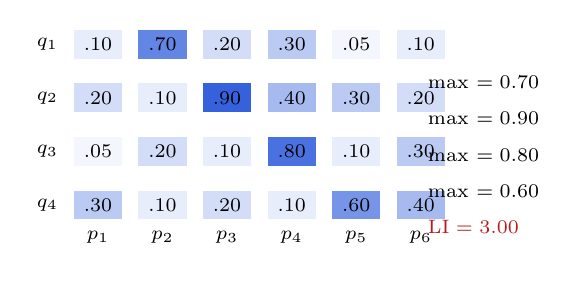
\begin{tikzpicture}[font=\scriptsize, x=0.82cm, y=0.68cm]
        \foreach \r/\vals in {0/{.10,.70,.20,.30,.05,.10},
                              1/{.20,.10,.90,.40,.30,.20},
                              2/{.05,.20,.10,.80,.10,.30},
                              3/{.30,.10,.20,.10,.60,.40}} {
          \foreach \c/\v [count=\ci from 0] in \vals {
            \pgfmathsetmacro{\shade}{int(\v*100)}
            \fill[blueaccent!\shade!white] (\ci,-\r) rectangle ++(0.78,0.58);
            \draw[white, thick] (\ci,-\r) rectangle ++(0.78,0.58);
            \node at (\ci+0.39,-\r+0.29) {\v};
          }
        }
        \foreach \r in {0,1,2,3} {
          \node[anchor=east] at (-0.08,-\r+0.29) {$q_{\the\numexpr\r+1\relax}$};
        }
        \foreach \c in {0,...,5} {
          \node[anchor=north] at (\c+0.39,-3.02) {$p_{\the\numexpr\c+1\relax}$};
        }
        \node[anchor=west, font=\scriptsize] at (5.35,-0.42) {max $=0.70$};
        \node[anchor=west, font=\scriptsize] at (5.35,-1.10) {max $=0.90$};
        \node[anchor=west, font=\scriptsize] at (5.35,-1.78) {max $=0.80$};
        \node[anchor=west, font=\scriptsize] at (5.35,-2.46) {max $=0.60$};
        \node[anchor=west, font=\scriptsize, text=mathred] at (5.35,-3.12) {$\mathrm{LI}=3.00$};
      \end{tikzpicture}

      \vspace{2mm}
      {\scriptsize Mỗi hàng = một token query; ô đậm = patch được chọn.}
    \end{column}
  \end{columns}
\end{frame}

% =============================================================
% SLIDE 11: LOSS
% =============================================================
\begin{frame}{Hàm mất mát: contrastive với hard negative}
  \begin{block}{\small Công thức (Eq.~2 trong paper)}
    \footnotesize
    Với batch $\{(q_k,d_k)\}_{k=1}^{b}$, đặt $s_k^{+}=\mathrm{LI}(q_k,d_k)$ và
    $s_k^{-}=\max_{l\neq k}\mathrm{LI}(q_k,d_l)$ (negative khó nhất trong batch):
    \[
      \mathcal{L}
      =-\frac{1}{b}\sum_{k=1}^{b}\log\frac{e^{s_k^{+}}}{e^{s_k^{+}}+e^{s_k^{-}}}
      =\frac{1}{b}\sum_{k=1}^{b}\log\!\left(1+e^{\,s_k^{-}-s_k^{+}}\right)
    \]
    Dạng \code{softplus} ổn định số học, tránh tràn khi $s^- - s^+$ lớn.
  \end{block}

  \vspace{2mm}
  \begin{columns}[T]
    \begin{column}{0.48\textwidth}
      \begin{block}{\small Vì sao hard negative?}
        \footnotesize
        Chỉ cần \emph{một} negative khó nhất: tín hiệu học mạnh, ít nhiễu hơn softmax trên toàn batch.
        Ablation ``No Pairwise'' (dùng toàn batch negatives) giảm 1.6 nDCG@5.
      \end{block}
    \end{column}
    \begin{column}{0.48\textwidth}
      \begin{block}{\small Lan truyền ngược}
        \footnotesize
        $\max$ và $\sum$ đều khả vi (max chọn nhánh) $\Rightarrow$ huấn luyện end-to-end qua cả LM và vision encoder.
        Thực tế paper chỉ mở LoRA ở LM + projection.
      \end{block}
    \end{column}
  \end{columns}
\end{frame}

% =============================================================
% SLIDE 12: TRAINING
% =============================================================
\begin{frame}{Huấn luyện: dữ liệu \& siêu tham số}
  \begin{columns}[T]
    \begin{column}{0.50\textwidth}
      \begin{block}{\small Dữ liệu}
        \footnotesize
        \textbf{118,695} cặp query--page:
        \begin{itemize}
          \item 63\% từ train set học thuật công khai;
          \item 37\% tổng hợp: PDF crawl web + câu hỏi giả do Claude-3 Sonnet sinh.
        \end{itemize}
        Hoàn toàn \textbf{tiếng Anh}; 2\% tách làm validation.\\
        Kiểm tra không trùng tài liệu với ViDoRe.
      \end{block}
      \begin{block}{\small Query augmentation}
        \footnotesize
        Thêm 5 token \code{<unused0>} vào query như ``soft query expansion''.
        Bỏ đi: tiếng Anh gần như không đổi, nhưng tiếng Pháp giảm mạnh (Shift $-9.8$, TabFQuAD $-6.3$).
      \end{block}
    \end{column}
    \begin{column}{0.46\textwidth}
      \begin{block}{\small Siêu tham số}
        \footnotesize
        \begin{tabular}{@{}ll@{}}
          Epoch & 1 \\
          Precision & bfloat16 \\
          LoRA & $r=32$, $\alpha=32$ \\
          Phạm vi LoRA & LM transformer + projection \\
          Optimizer & paged AdamW 8-bit \\
          LR & $5\times10^{-5}$, linear decay \\
          Warmup & 2.5\% \\
          Batch & 32 \\
          Phần cứng & 8 GPU, data parallel \\
        \end{tabular}
      \end{block}
      \begin{block}{\small Nhận xét}
        \footnotesize
        Chỉ 1 epoch trên 119k cặp --- nhỏ hơn nhiều so với contrastive pretraining của SigLIP.
      \end{block}
    \end{column}
  \end{columns}
\end{frame}

% =============================================================
% SLIDE 13: CHI PHI
% =============================================================
\begin{frame}{Chi phí: index, truy vấn, bộ nhớ}
  \begin{columns}[T]
    \begin{column}{0.50\textwidth}
      \begin{block}{\small Bộ nhớ (đánh đổi lớn nhất)}
        \footnotesize
        $1030\times128\times2$ byte $=\mathbf{257.5}$ KiB/trang.\\
        1 triệu trang $\approx$ 257 GB (chưa nén).\\
        So với bi-encoder 1 vector 1024 chiều: $\sim$2 KiB/trang --- gấp $\sim$125 lần.
      \end{block}
      \begin{block}{\small Token pooling}
        \footnotesize
        Gộp các patch trùng thông tin (nền trắng):
        pool $\times3$ $\Rightarrow$ giảm 66.7\% số vector, giữ 97.8\% hiệu năng.
        Tài liệu càng đặc chữ (Shift) càng kém chịu pooling.
      \end{block}
    \end{column}
    \begin{column}{0.46\textwidth}
      \begin{block}{\small Latency (NVIDIA L4)}
        \footnotesize
        \begin{tabular}{@{}ll@{}}
          ColPali query ($\sim$20 token) & 30 ms \\
          BGE-M3 query (15 token) & 22 ms \\
          Late interaction & 1 ms / 1000 tr. \\
          Index & 4 trang / batch \\
        \end{tabular}
      \end{block}
      \begin{block}{\small So với pipeline parse}
        \footnotesize
        Bỏ được layout detection + OCR + chunking + captioning.
        Trang được embed \emph{ngay} từ ảnh, throughput ổn định vì độ dài chuỗi cố định (1030 token).
      \end{block}
    \end{column}
  \end{columns}
\end{frame}

% =============================================================
% SLIDE 14: KET QUA VIDORE
% =============================================================
\begin{frame}{Kết quả ViDoRe: nDCG@5 theo task}
  \centering
  \scriptsize
  \setlength{\tabcolsep}{3.2pt}
  \begin{tabular}{@{}lrrrrrr@{}}
    \toprule
    Hệ thống & arXivQA & InfoVQA & TabFQuAD & TAT-DQA & Shift & \textbf{TB} \\
    \midrule
    SigLIP vanilla        & 43.2 & 64.1 & 58.1 & 26.2 & 18.7 & 51.4 \\
    BiSigLIP              & 58.5 & 70.5 & 62.7 & 30.5 & 26.5 & 58.6 \\
    BiPali                & 56.5 & 67.4 & 76.9 & 33.4 & 43.7 & 58.8 \\
    Unstructured+OCR (BGE-M3)      & 31.4 & 60.1 & 70.8 & 50.5 & 73.2 & 66.1 \\
    Unstructured+Captioning (BGE-M3) & 35.7 & 71.9 & 69.1 & 43.8 & 73.1 & 67.0 \\
    \midrule
    \textbf{ColPali}      & \good{79.1} & \good{81.8} & \good{83.9} & \good{65.8} & \good{73.2} & \good{81.3} \\
    \bottomrule
  \end{tabular}

  \vspace{4mm}
  \begin{columns}[T]
    \begin{column}{0.48\textwidth}
      \begin{block}{\small Nơi ColPali thắng đậm}
        \footnotesize
        arXivQA $+22.6$, InfoVQA $+14.4$, TabFQuAD $+7.0$ so với baseline mạnh nhất:
        đúng các task đòi hỏi đọc \emph{hình} và \emph{bảng}.
      \end{block}
    \end{column}
    \begin{column}{0.48\textwidth}
      \begin{block}{\small Nơi baseline còn cạnh tranh}
        \footnotesize
        Shift (văn bản dày, tiếng Pháp): 73.2 vs 73.1 --- gần như hòa.
        Nghĩa là visual retrieval không miễn nhiễm với văn bản thuần.
      \end{block}
    \end{column}
  \end{columns}
\end{frame}

% =============================================================
% SLIDE 15: ABLATION
% =============================================================
\begin{frame}{Ablation: cái gì thực sự tạo ra điểm?}
  \centering
  \footnotesize
  \begin{tabular}{@{}lrrl@{}}
    \toprule
    Biến thể & TB nDCG@5 & $\Delta$ & Diễn giải \\
    \midrule
    \textbf{ColPali (448px, 1024 patch)} & \textbf{81.3} & -- & tham chiếu \\
    ColPali 224px (256 patch)      & 56.5 & \hot{$-24.8$} & độ phân giải là yếu tố số 1 \\
    ColIdefics2 (64 patch)         & 76.6 & $-4.7$ & LLM 7B bù được ít patch \\
    ColQwen2 (768 patch)           & \good{86.6} & \good{$+5.3$} & backbone tốt hơn $\Rightarrow$ tốt hơn \\
    \midrule
    Chỉ train trên DocMatix        & 79.1 & $-2.2$ & vẫn hơn baseline $>12$ điểm \\
    Không query-aug tokens         & 79.6 & $-1.7$ & EN gần như đổi; FR giảm mạnh \\
    In-batch CE (thay pairwise)    & 79.7 & $-1.6$ & hard negative quan trọng \\
    Unfreeze vision encoder        & 80.6 & $-0.7$ & không cần thiết ở quy mô này \\
    + 1552 mẫu bảng tiếng Pháp     & 81.7 & $+0.4$ & TabFQuAD $+2.6$, Recall@1 $+5$ \\
    \bottomrule
  \end{tabular}

  \vspace{3mm}
  \begin{block}{\small Bài học}
    \footnotesize
    (1) Độ phân giải/patch count quan trọng hơn backbone; (2) late interaction là phần ``bùng nổ'' (BiPali $\rightarrow$ ColPali $+22.5$);
    (3) fine-tune rất rẻ và hiệu quả cho miền mới (chỉ 1552 mẫu đã $+2.6$).
  \end{block}
\end{frame}

% =============================================================
% SLIDE 16: INTERPRETABILITY
% =============================================================
\begin{frame}{Khả năng diễn giải: patch nào khớp token nào?}
  \begin{columns}[T]
    \begin{column}{0.50\textwidth}
      \begin{block}{\small Cách đọc heatmap}
        \footnotesize
        Với mỗi token query, tô đậm các patch có tích vô hướng cao nhất.
        Kết quả cho thấy ColPali \emph{định vị} được chữ và cả yếu tố phi chữ.
      \end{block}
      \begin{block}{\small Ví dụ trong paper}
        \footnotesize
        \begin{itemize}
          \item Token \code{<\_hour>} khớp cả ``hourly'' và ``hours'' $\Rightarrow$ có năng lực OCR mờ.
          \item Trục hoành của biểu đồ (đơn vị giờ) cũng được tô đậm.
          \item Token \code{<\_Kazakhstan>} khớp cả chữ ``Kashagan'' (mỏ dầu) $\Rightarrow$ có tri thức thế giới.
        \end{itemize}
      \end{block}
    \end{column}
    \begin{column}{0.46\textwidth}
      \centering
      \begin{tikzpicture}[font=\scriptsize]
        % page mock
        \draw[fill=white, draw=slateaccent] (0,0) rectangle (4.2,3.2);
        \node[anchor=north west, font=\tiny, text=slateaccent] at (0.1,3.1) {Bảng: thay đổi danh mục};
        % rows
        \foreach \y in {2.5,2.15,1.8,1.45,1.1} {
          \draw[slateaccent!40] (0.2,\y) -- (4.0,\y);
        }
        % highlighted patches
        \fill[mathred!35] (2.55,2.42) rectangle (3.35,2.72);
        \fill[mathred!35] (3.35,2.42) rectangle (4.05,2.72);
        \fill[blueaccent!30] (0.2,1.38) rectangle (1.05,1.68);
        \fill[mathgreen!30] (1.05,0.75) rectangle (2.0,1.05);
        \node[anchor=south, font=\tiny, text=mathred] at (3.3,2.73) {\code{<\_VPL>}};
        \node[anchor=south, font=\tiny, text=blueaccent] at (0.6,1.69) {\code{<\_ETF>}};
        \node[anchor=south, font=\tiny, text=mathgreen] at (1.5,1.06) {\code{<\_1,74>}};
      \end{tikzpicture}

      \vspace{1mm}
      {\scriptsize Mô phỏng: token $\rightarrow$ vùng ảnh.}
    \end{column}
  \end{columns}
\end{frame}

% =============================================================
% SLIDE 17: GIOI HAN
% =============================================================
\begin{frame}{Giới hạn cần nêu trung thực}
  \begin{columns}[T]
    \begin{column}{0.49\textwidth}
      \begin{block}{\small Về kỹ thuật}
        \footnotesize
        \begin{itemize}
          \item \textbf{Chỉ trả về trang}, không trả về đoạn/bảng cụ thể. Muốn RAG cần thêm bước patch $\rightarrow$ bounding box.
          \item 1030 vector/trang: index lớn hơn bi-encoder $\sim$125 lần.
          \item 3B tham số: khó chạy trên CPU/edge; 1 forward/trang vẫn đắt hơn embed text.
          \item Phụ thuộc độ phân giải: 224px mất 24.8 điểm.
        \end{itemize}
      \end{block}
    \end{column}
    \begin{column}{0.47\textwidth}
      \begin{block}{\small Về bằng chứng}
        \footnotesize
        \begin{itemize}
          \item Train set 100\% tiếng Anh; ViDoRe chỉ có Anh/Pháp $\Rightarrow$ tiếng Việt là \emph{zero-shot}.
          \item Benchmark 100--1600 ứng viên/task, chưa chứng minh ở quy mô triệu trang.
          \item Không sinh câu trả lời: vẫn cần LLM/VLM phía sau.
          \item So sánh công bằng khó: baseline parse dùng thiết lập mạnh nhất của paper.
        \end{itemize}
      \end{block}
    \end{column}
  \end{columns}

  \vspace{1mm}
  \begin{center}
    \footnotesize
    $\Rightarrow$ Câu hỏi cho đồ án: \emph{zero-shot ColPali có thắng BM25 trên bảng không kẻ tiếng Việt?}
  \end{center}
\end{frame}

% =============================================================
% SLIDE 18: THIET KE THUC NGHIEM
% =============================================================
\begin{frame}{Thực nghiệm: thiết kế trên corpus tiếng Việt}
  \begin{columns}[T]
    \begin{column}{0.52\textwidth}
      \begin{block}{\small Corpus \& gold set}
        \footnotesize
        \begin{itemize}
          \item 7 PDF đã parse: 3 broker forecast + 4 SSI review; 27 trang.
          \item 130 câu hỏi sinh từ 10 bảng (entity + value).
          \item Ví dụ: ``VPB được mua bao nhiêu triệu cổ phiếu bởi quỹ ETF mô phỏng VN30?'' $\rightarrow$ \texttt{1,74}.
        \end{itemize}
      \end{block}
      \begin{block}{\small Đơn vị đánh giá}
        \footnotesize
        \textbf{Page-level} (giống paper): mỗi câu hỏi có \textbf{1--3 trang vàng}
        (bảng trải trang). Trang vàng lấy từ text layer PyMuPDF, độc lập parser.
        Lý do: ColPali chỉ trả về trang; ép mọi hệ về cùng đơn vị để so sánh công bằng.
      \end{block}
    \end{column}
    \begin{column}{0.44\textwidth}
      \begin{block}{\small Hệ thống so sánh}
        \footnotesize
        \begin{enumerate}
          \item \textbf{BM25 trang}: text element của \texttt{unstructured} trên trang $\rightarrow$ BM25.
          \item \textbf{row-JSON / chipper / dual}: chunk $\rightarrow$ max-pool điểm lên trang.
          \item \textbf{ColPali / ColSmol}: ảnh trang $\rightarrow$ multi-vector $\rightarrow$ MaxSim.
        \end{enumerate}
      \end{block}
      \begin{block}{\small Metrics}
        \footnotesize
        Recall@$\{1,3,5,10\}$, MRR (trang); latency encode + query; dung lượng index.
      \end{block}
    \end{column}
  \end{columns}
\end{frame}

% =============================================================
% SLIDE 19: MOI TRUONG + CODE
% =============================================================
\begin{frame}[fragile]{Triển khai: CPU-only, không API}
  \begin{columns}[T]
    \begin{column}{0.40\textwidth}
      \begin{block}{\small Môi trường}
        \footnotesize
        \begin{itemize}
          \item Python 3.11, \code{colpali-engine}, PyMuPDF (150 DPI).
          \item Không GPU: \textbf{ColSmol-256M} (cùng late interaction, backbone nhỏ) cho lượt chạy đầy đủ.
          \item SmolVLM cắt trang A4 thành 13 crop $512\times512$ $\Rightarrow$ 875 vector/trang.
          \item Chạy thêm \textbf{ColPali-v1.2} trên subset để kiểm tra xu hướng.
        \end{itemize}
      \end{block}
      \begin{block}{\small Vì sao chấp nhận được?}
        \footnotesize
        Câu hỏi là \emph{so sánh tương đối} visual vs text retrieval, không phải tái lập SOTA.
      \end{block}
    \end{column}
    \begin{column}{0.56\textwidth}
      \begin{block}{\small Pipeline}
        \scriptsize
\begin{verbatim}
imgs  = render(pdf, dpi=150)
ds    = [{"image": im} for im in imgs]
E_d   = model.embed(ds)         # 875x128 (ColSmol)
E_q   = model.embed_queries([q]) # Nq x 128
score = maxsim(E_q, E_d).sum()
\end{verbatim}
      \end{block}
      \begin{block}{\small Lưu ý}
        \footnotesize
        Chuẩn hóa $L_2$ hai phía; dùng \code{ColPaliProcessor} để resize đúng 448px.
      \end{block}
    \end{column}
  \end{columns}
\end{frame}

% =============================================================
% SLIDE 20: KET QUA THUC NGHIEM (cap nhat sau khi chay)
% =============================================================
\begin{frame}{Kết quả trên corpus tiếng Việt}
  \centering
  \footnotesize
  \begin{tabular}{@{}lrrrrr@{}}
    \toprule
    Hệ thống (xếp hạng toàn bộ 27 trang) & R@1 & R@3 & R@5 & R@10 & MRR \\
    \midrule
    BM25 theo trang (\texttt{unstructured}) & 4.6 & 22.3 & 41.5 & 75.4 & 0.227 \\
    chipper\_prefix (max-pool)             & 45.4 & 89.2 & 99.2 & 100.0 & 0.665 \\
    dual\_small (max-pool)                 & 73.9 & 96.2 & 100.0 & 100.0 & 0.844 \\
    row\_json (max-pool)                   & \textbf{90.0} & \textbf{100.0} & \textbf{100.0} & \textbf{100.0} & \textbf{0.950} \\
    ColSmol-256M (zero-shot)               & 13.8 & 26.9 & 36.2 & 74.6 & 0.288 \\
    ColPali-v1.2 (zero-shot)               & \multicolumn{5}{c}{\textit{chưa chạy — cần GPU}} \\
    \bottomrule
  \end{tabular}

  \vspace{1mm}
  {\scriptsize \textit{Trang vàng lấy từ text layer PyMuPDF (1--3 trang/câu),
  không dùng trang bắt đầu bảng; vì thế số khác bản cũ.}}

  \vspace{2mm}
  \begin{columns}[T]
    \begin{column}{0.48\textwidth}
      \begin{block}{\small Đọc kết quả}
        \footnotesize
        Visual zero-shot \textbf{vượt BM25 trang} ở R@1 (13,8\% vs 4,6\%) ---
        tín hiệu ảnh có thật. Nhưng còn cách row-JSON \textbf{6,5 lần}
        (90,0\%) và dual\_small (73,9\%). Nguyên nhân: 256M, train tiếng Anh,
        27 trang bảng số gần như giống nhau.
      \end{block}
    \end{column}
    \begin{column}{0.48\textwidth}
      \begin{block}{\small Phạm vi từng file (27 trang $\rightarrow$ 3--6 trang)}
        \footnotesize
        BM25: R@1 17,7\%, MRR 0,528.\\
        ColSmol: R@1 20,8\%, MRR 0,547.\\
        Visual vượt BM25 ở R@1 nhưng vẫn rất thấp; đây là protocol dễ hơn,
        con số chính vẫn là corpus-level.
      \end{block}
    \end{column}
  \end{columns}
\end{frame}

% =============================================================
% SLIDE 21: KET LUAN
% =============================================================
\begin{frame}{Kết luận \& hướng tiếp theo}
  \begin{columns}[T]
    \begin{column}{0.49\textwidth}
      \begin{block}{\small Ba bài học từ paper}
        \footnotesize
        \begin{enumerate}
          \item Nút thắt của RAG tài liệu là \emph{ingestion}, không phải embedding model.
          \item Ảnh hóa tài liệu + late interaction cho phép bỏ hẳn parser/OCR/chunking.
          \item Độ phân giải (số patch) là đòn bẩy lớn nhất; fine-tune miền mới rất rẻ.
        \end{enumerate}
      \end{block}
    \end{column}
    \begin{column}{0.47\textwidth}
      \begin{block}{\small Hướng tiếp cho đồ án}
        \footnotesize
        \begin{itemize}
          \item Fine-tune LoRA ColPali trên cặp (câu hỏi, trang) tiếng Việt.
          \item Ánh xạ patch $\rightarrow$ bounding box để trả về đúng bảng (không chỉ trang).
          \item Thử ColQwen2 / ColSmol; nén index bằng token pooling.
          \item Kết hợp: visual retrieval lấy trang, row-JSON lấy ô --- hybrid 2 tầng.
        \end{itemize}
      \end{block}
    \end{column}
  \end{columns}
\end{frame}

% =============================================================
% SLIDE 22: TAI LIEU
% =============================================================
\begin{frame}{Tài liệu tham khảo}
  \footnotesize
  \begin{itemize}
    \item Faysse, Sibille, Wu, Omrani, Viaud, Hudelot, Colombo. \emph{ColPali: Efficient Document Retrieval with Vision Language Models}. ICLR 2025. arXiv:2407.01449.
    \item Khattab \& Zaharia. \emph{ColBERT: Efficient and Effective Passage Search via Contextualized Late Interaction over BERT}. SIGIR 2020.
    \item Beyer et al. \emph{PaliGemma: A Versatile 3B VLM for Transfer}. arXiv:2407.07726.
    \item Alabdulmohsin et al. \emph{SigLIP: Sigmoid Loss for Language Image Pre-training}. ICCV 2023.
    \item Clavié, Chaffin, Adams. \emph{Reducing the Footprint of Multi-Vector Retrieval with Minimal Performance Impact via Token Pooling}. arXiv:2409.14683.
    \item Faysse et al. \emph{ViDoRe benchmark \& leaderboard}. \url{https://huggingface.co/vidore}.
  \end{itemize}

  \vspace{3mm}
  \begin{block}{\small Ghi chú số liệu}
    \footnotesize
    Mọi con số ở Phần I--II lấy từ arXiv:2407.01449v3 (Table 2, 6, 7).
    Số ở Phần III do đồ án tự đo trên corpus riêng, \textbf{không} so sánh trực tiếp với ViDoRe.
  \end{block}
\end{frame}

\end{document}
